% F092｜高中数学常用数值表｜04_examples.tex
% 继承上传模板的 LaTeX 环境；当前条目的内容独立编写。
\clearpage
\begin{examplebox}
\textbf{\textcolor{CExample}{例 1：快速估算根号6}}
\par\medskip
\begin{center}
% F092｜cards 原创简明教学示意图
\begin{tikzpicture}[>=stealth,scale=.92]
\node[draw,rounded corners,fill=teal!9,minimum width=2.7cm,minimum height=1.2cm] at (0,0){$\sqrt2\approx1.414$};
\node[draw,rounded corners,fill=orange!9,minimum width=2.7cm,minimum height=1.2cm] at (3.1,0){$\ln2\approx0.693$};
\node[draw,rounded corners,fill=teal!9,minimum width=2.7cm,minimum height=1.2cm] at (6.2,0){$e\approx2.718$};
\node at (3.2,-1.0){\small 先记少数基准数，其余借公式推导};
\end{tikzpicture}

\end{center}
\medskip
$\sqrt6=\sqrt2\sqrt3$；用表 $1.414\times1.732\approx2.449$。\textbf{提醒：}末位由输入精度影响，严谨计算应保留中间精度后再舍入。
\end{examplebox}
\clearpage
\begin{examplebox}
\textbf{\textcolor{CExample}{例 2：快速求lg5}}
\par\medskip
\begin{center}
% F092｜derive 原创简明教学示意图
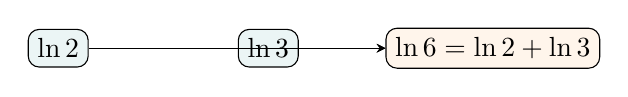
\begin{tikzpicture}[>=stealth,scale=.92]
\node[draw,rounded corners,fill=teal!8] (a) at (0,0){$\ln2$};
\node[draw,rounded corners,fill=teal!8] (b) at (2.9,0){$\ln3$};
\node[draw,rounded corners,fill=orange!8] (c) at (6,0){$\ln6=\ln2+\ln3$};
\draw[->] (a)--(c);\draw[->] (b)--(c);
\end{tikzpicture}

\end{center}
\medskip
$\lg5=\lg(10/2)=1-\lg2\approx1-0.301=0.699$。比背一张全表更轻松。
\end{examplebox}
\clearpage
\begin{examplebox}
\textbf{\textcolor{CExample}{例 3：由勾股数判断斜边}}
\par\medskip
\begin{center}
% F092｜square 原创简明教学示意图
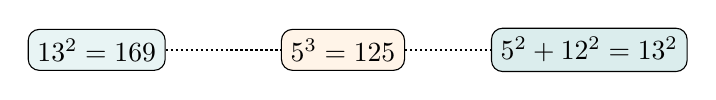
\begin{tikzpicture}[>=stealth,scale=.92]
\node[draw,rounded corners,fill=teal!9] (a) at (0,0){$13^2=169$};
\node[draw,rounded corners,fill=orange!9] (b) at (3.4,0){$5^3=125$};
\node[draw,rounded corners,fill=teal!14] (c) at (6.8,0){$5^2+12^2=13^2$};
\draw[densely dotted,thick] (a)--(b);\draw[densely dotted,thick] (b)--(c);
\end{tikzpicture}

\end{center}
\medskip
两直角边分别是 $5$ 和 $12$，用 $5^2+12^2=25+144=169=13^2$，得斜边 $13$。可直接联系表中的 $13^2$。
\end{examplebox}
